  \begin{subfigure}{\textwidth}
    \centering
  \begin{tabular}[c]{|c|c|}
    \multicolumn{2}{c}{$S_a$} \\ \hline
    $t$  & $v$ \\ \hline
    0   & 0 \\
    2   & 1 \\
    4   & 3 \\
    5   & 4 \\
    8   & 10 \\ \hline
  \end{tabular} \qquad
  \begin{tabular}[c]{|c|c|}
    \multicolumn{2}{c}{$S_\Delta$} \\ \hline
    $t$  & $v$ \\ \hline
    0   & 0 \\
    2 & 1 \\
    4 & 2 \\
    5 & 1 \\
    8 & 6 \\ \hline
  \end{tabular} \qquad
  \begin{tabular}[c]{|c|c|}
    \multicolumn{2}{c}{$S_v$} \\ \hline
    $t$  & $v$ \\ \hline
    0   & 0 \\
    2 & 0{,}5 \\
    4 & 1 \\
    5 & 1 \\
    8 & 2 \\ \hline
  \end{tabular}
  \caption{Taules de valors}
  \end{subfigure}

  \begin{subfigure}{0.3\textwidth}
  \begin{tikzpicture}
    \begin{axis}[
        timeseriesrel,
        title=$S_a$,
        ]
    \addplot[blue] coordinates {
        (0,0)
        (2,1)
        (4,3)
        (5,4)
        (8,10)
    };
    %\addlegendentry{Valor absolut}
    \addplot[only marks,mark=*,red] coordinates {
        (0,0)
        (2,1)
        (4,3)
        (5,4)
        (8,10)
    };
    % \addlegendentry{Punts de mesura}
    \end{axis}
  \end{tikzpicture}
  \caption{Valor absolut}
  \end{subfigure}
  \begin{subfigure}{0.3\textwidth}
  \begin{tikzpicture}
    \begin{axis}[
        timeseriesrel,
        title=$S_\Delta$,
        ]
    \addplot[ycomb,blue,mark=-] coordinates {
        (0,0)
        (2,1)
        (4,2)
        (5,1)
        (8,6)
    };
    %\addlegendentry{Increments}
    \addplot[only marks,mark=*,red] coordinates {
        (0,0)
        (2,1)
        (4,2)
        (5,1)
        (8,6)
    };
    %\addlegendentry{Punts de mesura}

    \addplot[gray,dashed] coordinates {
        (0,0)
        (2,1)
        (4,2)
        (5,1)
        (8,6)
    };
    % \addlegendentry{Tendència}

    \end{axis}
  \end{tikzpicture}
  \caption{Increments}
  \end{subfigure}
 \begin{subfigure}{0.3\textwidth}
  \centering
  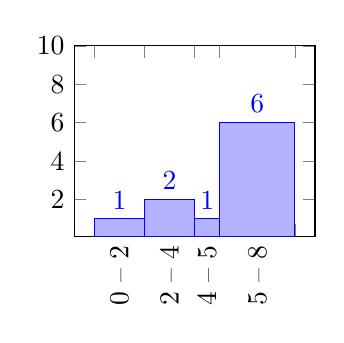
\begin{tikzpicture}
    \begin{axis}[
%        timeseriesrel,
        height=4cm,
        %width=10cm,scale only axis, height=5cm,
        ymax = 10,
        xtick = data,
        xticklabel interval boundaries,
        x tick label style= {rotate=90,anchor=east},
        x label style ={ at={(1,0)},left,yshift=0pt},
        ]
    \addplot[ybar interval,blue,fill=blue!30!white] coordinates{
        (0,1)
        (2,2)
        (4,1)
        (5,6)
        (8,6)
    }; 
    % \addlegendentry{Increments}

    \node[color=blue,above] at (axis cs:1,1) {1};
    \node[color=blue,above] at (axis cs:3,2) {2};
    \node[color=blue,above] at (axis cs:4.5,1) {1};
    \node[color=blue,above] at (axis cs:6.5,6) {6};
    \end{axis}
  \end{tikzpicture}
  \caption{Gràfic de barres}
  \end{subfigure}

  \begin{subfigure}{0.3\textwidth}
  \centering
  \begin{tikzpicture}
    \begin{axis}[
        timeseriesrel,
        title=$S_\Delta$
        ]
    \addplot[blue] coordinates {
        (0,0)
        (2,1)
        (2,0)
        (4,2)
        (4,0)
        (5,1)
        (5,0)
        (8,6)
        (8,0)
    };
    %\addlegendentry{Valor relatiu}
    \addplot[only marks,mark=*,red] coordinates {
        (0,0)
        (2,1)
        (4,2)
        (5,1)
        (8,6)
    };
    %\addlegendentry{Punts de mesura}
    \end{axis}
  \end{tikzpicture}
  \caption{Valor relatiu}
  \end{subfigure}
  \begin{subfigure}{0.3\textwidth}
  \centering
  \begin{tikzpicture}
    \begin{axis}[
        timeseriesrel,
        title=$S_v$,
        ]
    \addplot[const plot mark right,blue] coordinates {
        (0,0)
        (2,0.5)
        (4,1)
        (5,1)
        (8,2)
    };
    %\addlegendentry{Velocitat mitjana}

   \addplot[only marks,mark=*,red] coordinates {
        (0,0)
        (2,0.5)
        (4,1)
        (5,1)
        (8,2)
    };
    %\addlegendentry{Punts de mesura}

    \end{axis}
  \end{tikzpicture}
  \caption{Velocitat}
   \end{subfigure}
  \begin{subfigure}{0.3\textwidth}
  \centering
  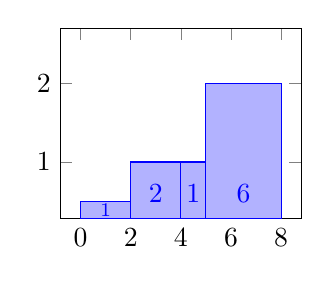
\begin{tikzpicture}
    \begin{axis}[
        height=4cm,
        ymax=2.7,
        ]
    \addplot[ybar interval,blue,fill=blue!30!white,mark=none] coordinates {
        (0,0.5)
        (2,1)
        (4,1)
        (5,2)
        (8,2)
    };
    %\addlegendentry{distribució d'increments}

    \node[color=blue] at (axis cs:1,0.39) {\scriptsize 1};
    \node[color=blue] at (axis cs:3,0.6) {2};
    \node[color=blue] at (axis cs:4.5,0.6) {1};
    \node[color=blue] at (axis cs:6.5,0.6) {6};
     \end{axis}
  \end{tikzpicture}
  \caption{Histograma}
  \end{subfigure}
